\documentclass{article}


\usepackage{arxiv}

\usepackage[utf8]{inputenc} % allow utf-8 input
\usepackage[T1]{fontenc}    % use 8-bit T1 fonts
\usepackage{hyperref}       % hyperlinks
\usepackage{url}            % simple URL typesetting
\usepackage{booktabs}       % professional-quality tables
\usepackage{amsfonts}       % blackboard math symbols
\usepackage{nicefrac}       % compact symbols for 1/2, etc.
\usepackage{microtype}      % microtypography
\usepackage{lipsum}
\usepackage{enumitem}
\usepackage[polish]{babel} % English language hyphenation
\usepackage{float} % for H in \begin{figure}[H]. Force including file in place.

\usepackage{graphicx}
\graphicspath{ {./images/} }

\fancyhf{} % sets both header and footer to nothing
\renewcommand{\headrulewidth}{0pt}
% your new footer definitions here


% kolory odnośników
\usepackage[dvipsnames]{xcolor}
\hypersetup{
    colorlinks=true,
    linkcolor=black,
    filecolor=black,
    citecolor=black,
    urlcolor=cyan,
    pdftitle={Sharelatex Example},
    pdfpagemode=FullScreen,
}
\urlstyle{same}


\title{Kwantyzacja wektorowa}

\author{
  Karol Działowski \\
  \textbf{Wojciech Olejnik} \\
  \textbf{Paweł Kalicki} \\
  Zachodniopomorski Uniwersytet Technologiczny
}

\begin{document}
\maketitle
\begin{abstract}
Lorem Ipsum is simply dummy text of the printing and typesetting industry. Lorem Ipsum has been the industry's standard dummy text ever since the 1500s, when an unknown printer took a galley of type and scrambled it to make a type specimen book. It has survived not only five centuries, but also the leap into electronic typesetting, remaining essentially unchanged. It was popularised in the 1960s with the release of Letraset sheets containing Lorem Ipsum passages, and more recently with desktop publishing software like Aldus PageMaker including versions of Lorem Ipsum. Do implementacji aplikacji wykorzystano język programowania Python.
\end{abstract}


% keywords can be removed
%\keywords{First keyword \and Second keyword \and More}


\section{Wstęp}

Kwantyzacja polega na przyporządkowaniu wartościom sygnału z jakiegoś określonego ciągłego przedziału wartości dyskretnych z przyjętego skończonego zbioru. Maksymalna wartość sygnału dzielona jest na szereg drobniejszych przedziałów. Zazwyczaj przedziały mają taką samą wielkość (jest to kwantyzacja liniowa), ale są wyjątki od tej reguły i niekiedy stosuje się kwantyzację nieliniową. Z każdym przedziałem powiązana jest określona liczba. Jeśli wielkość sygnału wejściowego mieści się w danym przedziale, to wówczas jest ona reprezentowana przez liczbę związaną z tym przedziałem.

Proces kwantyzacji sygnału jest zaokrąglany i w rezultacie powstają błędy. Błędy te objawiają się w postaci tak zwanego szumu kwantyzacji. Im większe przedziały kwantyzacji, tym mniejsza jej dokładność i tym większy szum kwantyzacji. W przetwarzaniu analogowo-cyfrowym dokładność liniowej kwantyzacji jest określona przez ilość bitów wykorzystywanych do zapisu skwantowanej wartości. Zwiększenie ilości bitów prowadzi do zwiększenia ilości przedziałów i dokładniejszego odwzorowania sygnału \cite{drozdek2007wprowadzenie}.

\section{Opis projektu}

Celem projektu było stworzenie aplikacji umożliwiającej przeprowadzanie kwantyzacji wektorowej.

\subsection{Kwantyzacja wektorowa}
Kwantyzacja wektorowa (\textit{ang. vector quantization}) to przypisanie jednego słowa kodowego do grupy dwóch lub więcej elementów obrazu. Kompresja jest osiągana dzięki liczbie dostępnych słów kodowych mniejszej niż liczba permutacji możliwych wartości pikseli wejściowych w grupie. W ten sposób kilka wzorców wejściowych jest mapowanych na jeden kod wyjściowy. To ponownie wykorzystuje prawdopodobne podobieństwa między pikselami w tym samym sąsiedztwie przestrzeni lub czasu lub obu i maskowanie zniekształceń w bardzo szczegółowych obszarach.
\begin{figure}[H]
    \centering
    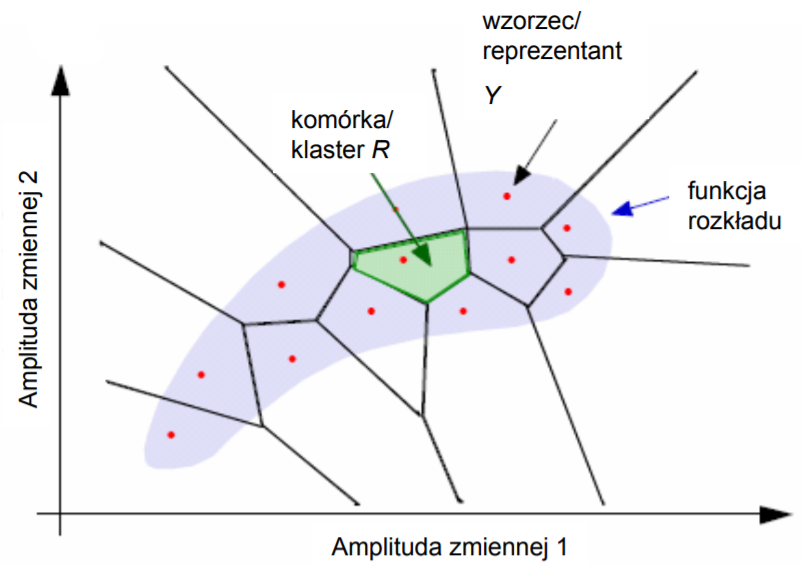
\includegraphics[width=0.6\textwidth]{images/kwantyzacja_wektorowa.png}
    \caption{Przykład podziału dwuwymiarowej przestrzeni danych na klastry grupujące według słownika. Źródło \cite{mwilczewski}}
    \label{fig:crossing}
\end{figure}

\subsection{Ogólny przebieg etapów pracy kwantyzatora wektorowego}

\begin{enumerate}
  \item Formowanie danych wejściowych do postaci N wektorów n-wymiarowych (etap wstępny). 
  \item Faza klasteryzacji: podział wszystkich wektorów wejściowych i konstrukcja książki kodowej (słownika) zawierającej K najbardziej reprezentatywnych wektorów całego zbioru danych, tzw. wektorów kodowych. Konstrukcja książki kodowej może być wykonana w fazie wstępnej na podstawie zbioru treningowego lub dynamicznie we właściwej fazie kwantyzacji. Faza klasteryzacji jest kluczowym etapem kwantyzacji wektorowej.
  \item Faza indeksowania: przyporządkowanie każdemu wektorowi wejściowemu jednego wektora ze słownika i reprezentowanie wektora wejściowego indeksem słownika. 
\end{enumerate}

\begin{figure}[H]
    \centering
    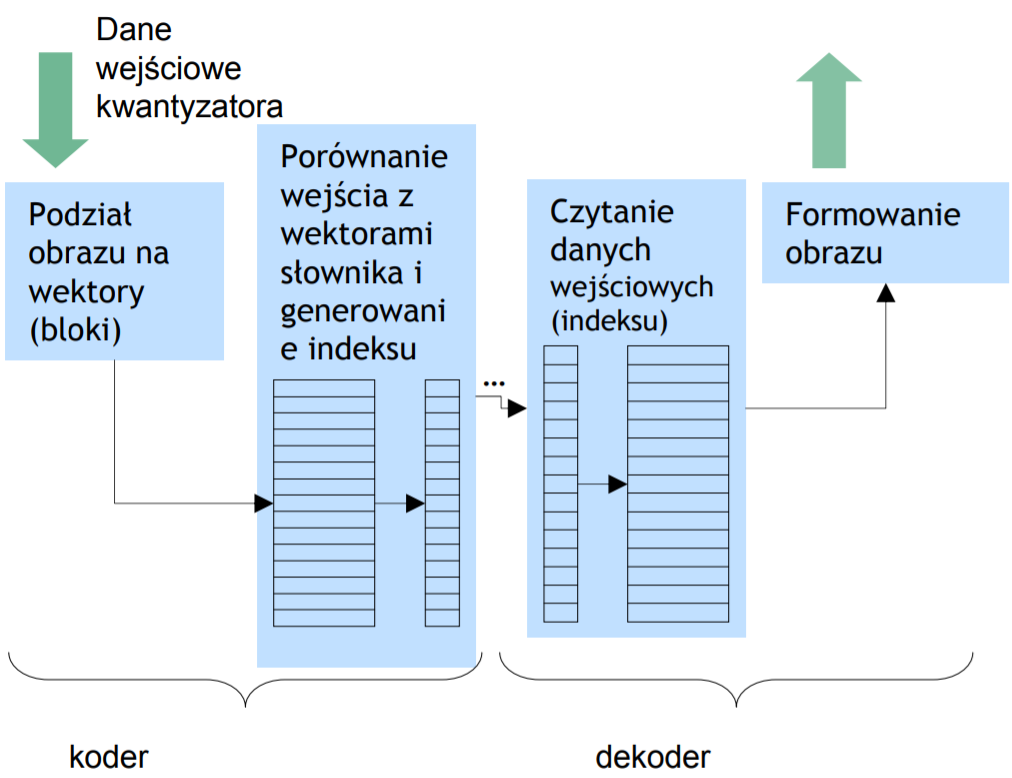
\includegraphics[width=0.6\textwidth]{images/schemat_kwantyzatora.png}
    \caption{Ogólny schemat pracy kwantyzatora. Źródło \cite{mwilczewski}}
    \label{fig:crossing}
\end{figure}

\begin{figure}[H]
    \centering
    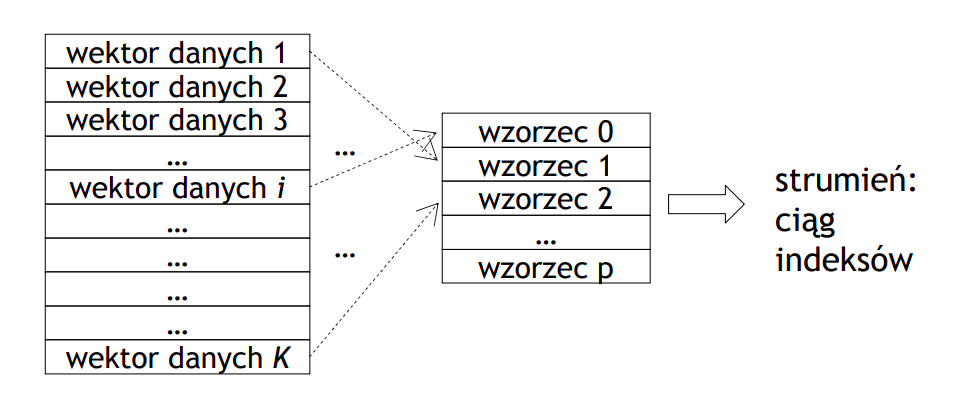
\includegraphics[width=0.6\textwidth]{images/wektory_danych.png}
    \caption{Porównywanie wektorów danych z wektorami ze słownika. Źródło \cite{mwilczewski}}
    \label{fig:crossing}
\end{figure}

Problemy jakie możemy napotkać podczas kwantyzacji wektorowej:
\begin{enumerate}
  \item Wybór odpowiedniej funkcji odległości w przestrzeni wektorowej.  
  \item Struktura książki kodowej (prosta struktura w postaci tablicy jest nieefektywna do przeglądania).
\end{enumerate}

\subsection{Inicjalizacja książki kodowej}

W procesie kwantyzacji wektorowej ważna rolę odgrywa postać książki kodowej ze względu na zbieżność do lokalnego minimum błędu kwantyzacji. Podstawowymi metodami inicjalizacji książki kodowej :

\begin{enumerate}
  \item metoda losowania,
  \item metoda grupowania najbliższych sąsiadów (ang. PNN - pairwise nearest neighbour)
  \item metoda rozdzielania (ang. splitting) 
\end{enumerate}

Pierwsza z wymienionych powyżej, czyli metoda losowa polega na wylosowaniu N wektorów, gdzie N jet liczba całkowitą. Oczywiście takie rozwiązanie jest odpowiednie, wtedy gdy nie mamy informacji na temat danych wektorowych. Posiadając informacje możemy wykorzystać ją do zawężenia obszaru losowego.

Druga metoda tworzenie słownika, czyli metoda grupowania pozwala osiągnąć lepsze wyniki niż metoda losowa, ale za to jest nieco bardziej czasochłonna. Polega ona na tworzeniu coraz liczniejszych grup zaczynając od jednoelementowej, związanej z każdym wektorem sekwencji. W następnych iteracjach wyznaczamy najbliższe grupy, czyli liczymy odległości pomiędzy środkami poszczególnych grup. Następnie dwie najbliższe sobie grupy zostają połączone tak aby zmniejszać liczbe grup.

Ostatnia wymieniona metoda jaką jest metoda rozdzielania - polega na szukaniu optymalnej książki. Konstrukcja rozpoczyna się od pojedynczego wektora – centroidu zbioru uczącego. W i-tym kroku dokonywany jest (w drodze dodawania zaburzenia) podział każdego z wektorów kodowych na dwa wektory. Po takim rozdzieleniu uzyskana konfiguracja regionów decyzyjnych jest optymalizowana przez algorytm LBG, po czym dokonywany jest kolejny rozdział, etc.

\begin{figure}[H]
    \centering
    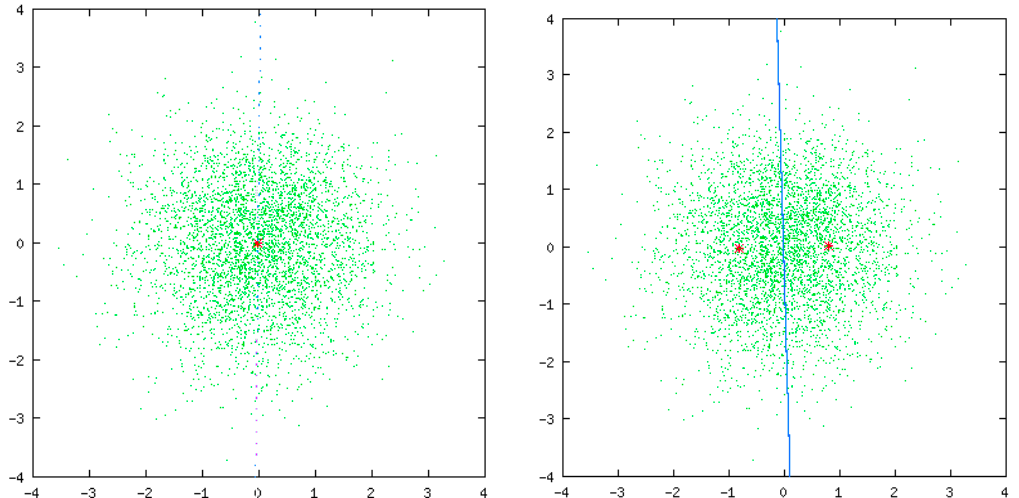
\includegraphics[width=0.6\textwidth]{images/rodzielania_1.png}
    \caption{Konstrukcja słownika metodą rozdzialania. Kolejne etapy konstrukcji wektorów kodowych (zaznaczone czerwonymi punktami) na zbiorze uczącym (zaznaczony kolorem zielonym).  Źródło \cite{mwilczewski}}
    \label{fig:crossing}
\end{figure}

\begin{figure}[H]
    \centering
    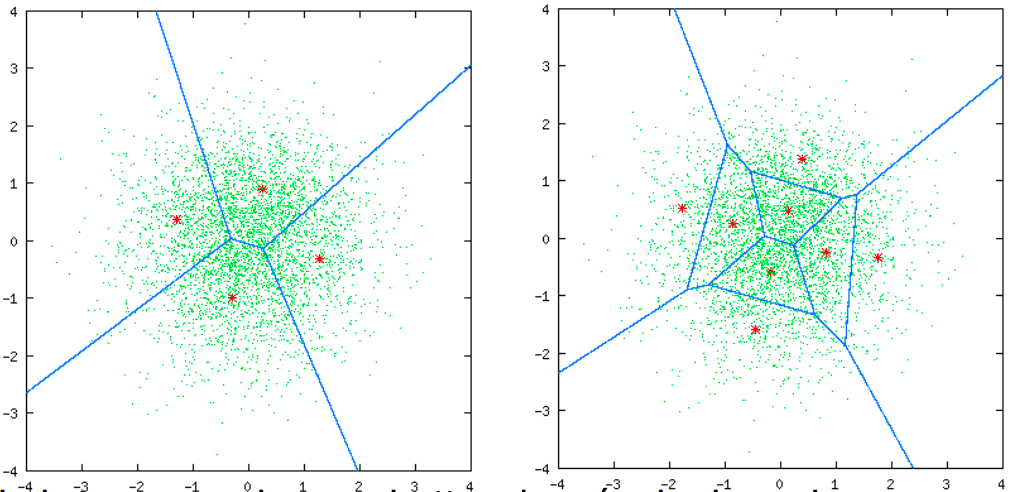
\includegraphics[width=0.6\textwidth]{images/rodzielania_2.png}
    \caption{Konstrukcja słownika metodą rozdzialania. Kolejne etapy konstrukcji wektorów kodowych (zaznaczone czerwonymi punktami) na zbiorze uczącym (zaznaczony kolorem zielonym).  Źródło \cite{mwilczewski}}
    \label{fig:crossing}
\end{figure}

\subsection{Algorytmy inicjalizowania słownika}

\subsubsection{Algorytm popularności}

Algorytm popularności jest prostym algorytmem generacji książki kodowej, który charakteryzuje się:

\begin{itemize}
  \item wektorami kodowymi staje się ustalona liczba wektorów danych występujących w obrazie najczęściej (konieczne jest ustalenie progu liczby wystąpień) 
  \item algorytm wyróżnia się stosunkowo małą złożonością obliczeniową i prostotą implementacji 
  \item wadą podstawowej wersji algorytmu popularności jest wprowadzanie do książki kodowej podobnych barw (dominujących). Redukcję rozmiaru książki uzyskać można przez usunięcie bliskich (w sensie przyjętej metryki) wektorów i wprowadzenie kolejnego wektora pod względem liczby wystąpień. 

\begin{figure}[H]
    \centering
    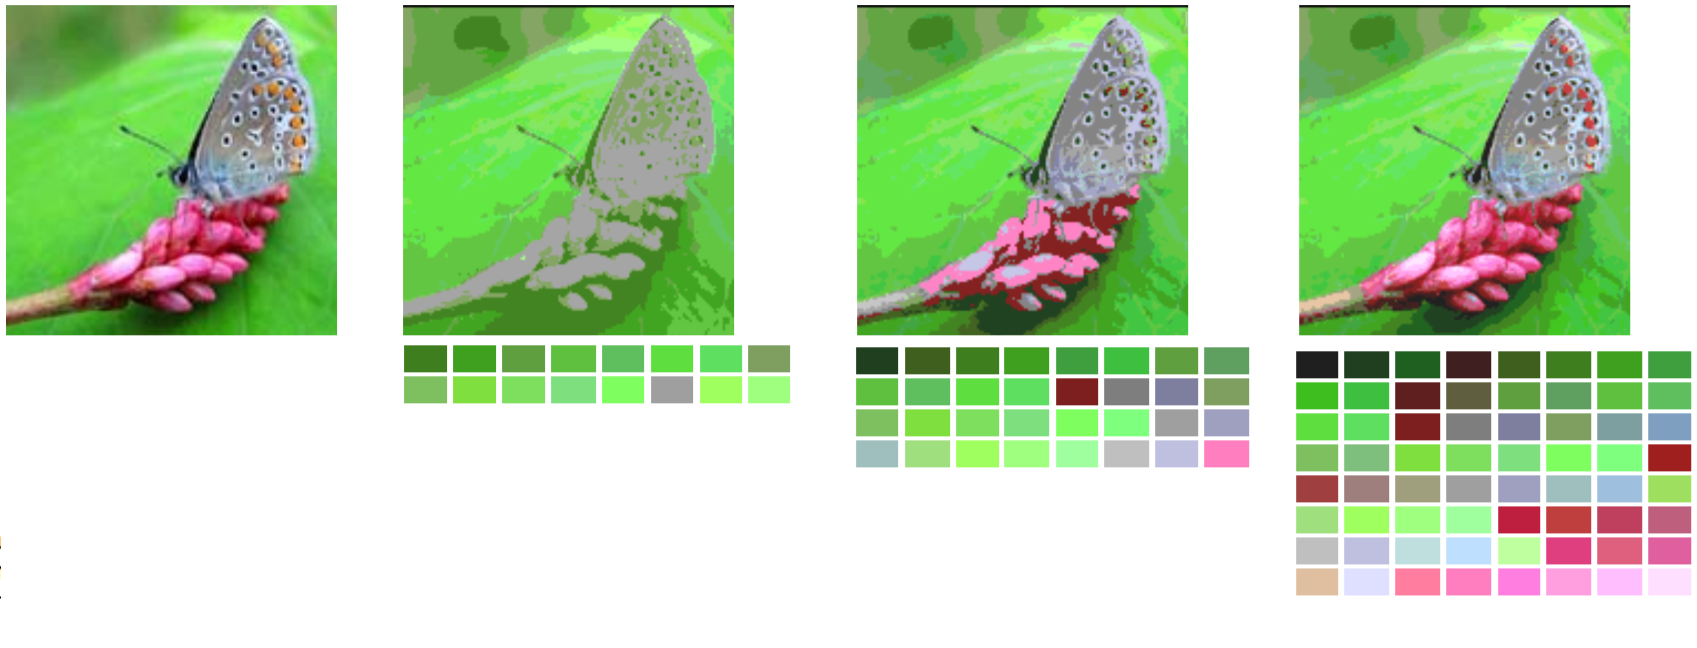
\includegraphics[width=0.6\textwidth]{images/motyle_2.png}
    \caption{Przykład kwantyzacji wektorowej przeprowadzonej z książką kodową skonstruowaną zgodnie z algorytmem popularności. Efekt kwantyzacji wektorowej z książkami kodowymi
rozmiaru odpowiednio: 16, 32 oraz 64. Źródło \cite{aprzelaskowski}}
    \label{fig:crossing}
\end{figure}
 
\end{itemize}

\subsubsection{Wektorowa kwantyzacja blokowa (BTC)}

Wektorowa kwantyzacja blokowa (BTC) charakteryzuje się:

\begin{itemize} 
\item W przypadku podstawowej wersji metody BTC każdy skwantyzowany blok obrazu reprezentowany jest w strumieniu bitowym przez mapę bitową zawierającą $n^{2} = n \times n$ bitów oraz dwa bajty reprezentujące poziomy rekonstrukcji. W takim przypadku:
     \begin{itemize}[label=$\star$]
        \item liczba wszystkich możliwych map bitowych jest równa $n^{2}$ = 65536,
        \item nie wszystkie z nich występują w każdym obrazie cyfrowym, np. ze względu na rozmiar obrazu oraz korelacje danych obrazowych, 
     \end{itemize}
\item jednym z możliwych sposobów wykorzystania powyższych obserwacji do kompresji obrazu jest kwantyzacja wektorowa map bitowych, tzn. reprezentacja zbioru wszystkich możliwych map bitowych przez niewielki jego podzbiór (słownik),
\item w fazie indeksacji, każda z map bitowych stworzonych dla kolejnych bloków obrazu porównywana jest ze zbiorem map w słowniku. Prostą miarą podobieństwa map jest liczba miejsc na których porównywane mapy różnią się. Mapą najbardziej podobną do zadanej jest mapa minimalizująca tak zdefiniowaną miarę,
\item wykorzystanie zbioru map stanowiących słownik zwiększa stopień kompresji. Przykład: w przypadku bloków 4x4 oraz 32 elementowego słownika 16 bitów reprezentujących elementy oryginalnej mapy można zastąpić 5 bitowym indeksem słownika. Zwiększa to stopień kompresji z CR=4.0 do CR=6.09.
\end{itemize}

\subsubsection{Algorytm Lindego-Buza-Graya}

Algorytm Lindego-Buza-Graya (LBG), powstał 1980, służy od do generowania książki kodowej. Przebieg algorytmu przedstawia się następująco:

\begin{itemize} 
\item określ wektory danych zbioru uczącego. Spośród wszystkich N wektorów wejściowych wybierz losowo K wektorów stanowiących wstępną wersję słownika,
\item korzystając metryki euklidesowej, d(X,Y), dokonaj klasteryzacji wektorów danych wokół słów kodowych bieżącej wersji słownika
     \begin{itemize}[label=$\star$]
        \item bierzemy każdy kwadrat z obrazu (4x4) i sprawdzamy któremu reprezentantowi ze słownika jest najbliżej do naszego kwadratu, każdy piksel wewnątrz tego kwadratu porównujemy ze sobą i liczymy ich różnice w kwadracie ,
        \item następnie sumujemy różnic 16 kwadratów
        \item sprawdzamy kwadrat z obrazu z każdym reprezentantem słownika centroid
        \item przypisujemy wybrany kwadrat do reprezentanta słownika
     \end{itemize}
\item wyznacz globalny błąd kwantyzacji popełniony w bieżącej iteracji czyli wykonujemy sumowanie wszystkich znalezionych odległości miedzy poszczególnymi kwadratami a centroidami 
 
\begin{equation}
e = \sum_{i=1}^K \sum_{x\in\mathbb{R}} d(X, Y_{i}) 
\end{equation}

\item sprawdzić czy popełniany błąd zmienił się względem poprzedniej iteracji jeśli nie ma to zakończ algorytm (dla uproszczenia ustaliliśmy, że ilość iteracji będzie podawana z ręki)
\item wyznacz centroidy każdego regionu decyzyjnego i uczyń je wektorami kodowymi kolejnej iteracji słownika. Przejdź do kroku 2. 
\end{itemize}
 
Problemy tego algorytmu:

\begin{itemize}
	\item wrażliwość na inicjalną postać książki kodowej 
	\item problem pustych przedziałów 
\end{itemize}

\subsection{PSNR}

Szczytowy stosunek sygnału do szumu, (ang. peak signal-to-noise ratio ( PSNR) ) – stosunek maksymalnej mocy sygnału do mocy szumu zakłócającego ten sygnał.  

Najczęściej PSNR stosowany jest do oceny jakości kodeków wykorzystujących stratną kompresję obrazków. W takim przypadku sygnałem są nieskompresowane dane źródłowe, a szumem – artefakty (zniekształcenia) spowodowane zastosowaniem kompresji stratnej. 

W celu wyznaczenie PSNR, należy najpierw obliczyć współczynnik MSE (błąd średniokwadratowy) bazując na obu porównywanych obrazkach za pomocą wzoru:

\begin{equation}
MSE = \frac{1}{N * M} \sum_{i=1}^N \sum_{j=1}^M ([f(i, j) - f^{'}(i, j)]^2
\end{equation}

gdzie:
\begin{itemize}[label=]
    \item $N, M$ - wymiary obrazu w pikselach,
    \item $f(i, j)$ - wartość piksela o współrzędnych $i(i, j)$ obrazu oryginalnego
    \item $f^{'}(i, j)$ - wartość piksela o współrzędnych $i(i, j)$ obrazu skompresowanego
\end{itemize}

Następnie wyliczoną wartość MSE należy podstawić do końcowego wzoru: 

\begin{equation}
PSNR = 10 * \log_10 \frac{[max(f(i,j))]^2}{MSE}
\end{equation}

gdzie:
\begin{itemize}[label=]
    \item $max(f(i,j))$ - wartość maksymalna danego sygnału; w przypadku obrazów zwykle jest to wartość stała, np. dla obrazów monochromatycznych o reprezentacji 8-bitowej wynosi 255.
\end{itemize}

\section{Podsumowanie}

Lorem Ipsum is simply dummy text of the printing and typesetting industry. Lorem Ipsum has been the industry's standard dummy text ever since the 1500s, when an unknown printer took a galley of type and scrambled it to make a type specimen book. It has survived not only five centuries, but also the leap into electronic typesetting, remaining essentially unchanged. It was popularised in the 1960s with the release of Letraset sheets containing Lorem Ipsum passages, and more recently with desktop publishing software like Aldus PageMaker including versions of Lorem Ipsum. Do implementacji aplikacji wykorzystano język programowania Python.

Lorem Ipsum is simply dummy text of the printing and typesetting industry. Lorem Ipsum has been the industry's standard dummy text ever since the 1500s, when an unknown printer took a galley of type and scrambled it to make a type specimen book. It has survived not only five centuries, but also the leap into electronic typesetting, remaining essentially unchanged. It was popularised in the 1960s with the release of Letraset sheets containing Lorem Ipsum passages, and more recently with desktop publishing software like Aldus PageMaker including versions of Lorem Ipsum. Do implementacji aplikacji wykorzystano język programowania Python.

\bibliographystyle{unsrt}  
\bibliography{references}  %%% Remove comment to use the external .bib file (using bibtex).
%% and comment out the ``thebibliography'' section.

\end{document}
